\section{مقدمه و تعریف DevOps}
DevOps یک فرهنگ، فلسفه و مجموعه‌ای از روش‌ها و ابزارها است که هدف اصلی آن، یکپارچه‌سازی و خودکارسازی فرآیندهای بین تیم‌های توسعه نرم‌افزار (Development) و عملیات فناوری اطلاعات (Operations) است. در مدل سنتی، این دو تیم جدا از هم عمل می‌کردند که منجر به کندی، خطاهای بیشتر و هماهنگی دشوار می‌شد. ظهور DevOps پاسخی به این چالش‌ها بود تا با ایجاد همکاری و مسئولیت مشترک، شکاف بین ساخت نرم‌افزار و اجرای پایدار آن را از بین ببرد. در نهایت، DevOps به سازمان‌ها این توانایی را می‌دهد که نرم‌افزارها را سریع‌تر، قابل‌اطمینان‌تر و با کیفیت بالاتر در اختیار کاربران قرار دهند.

\begin{figure}[h]
\centering
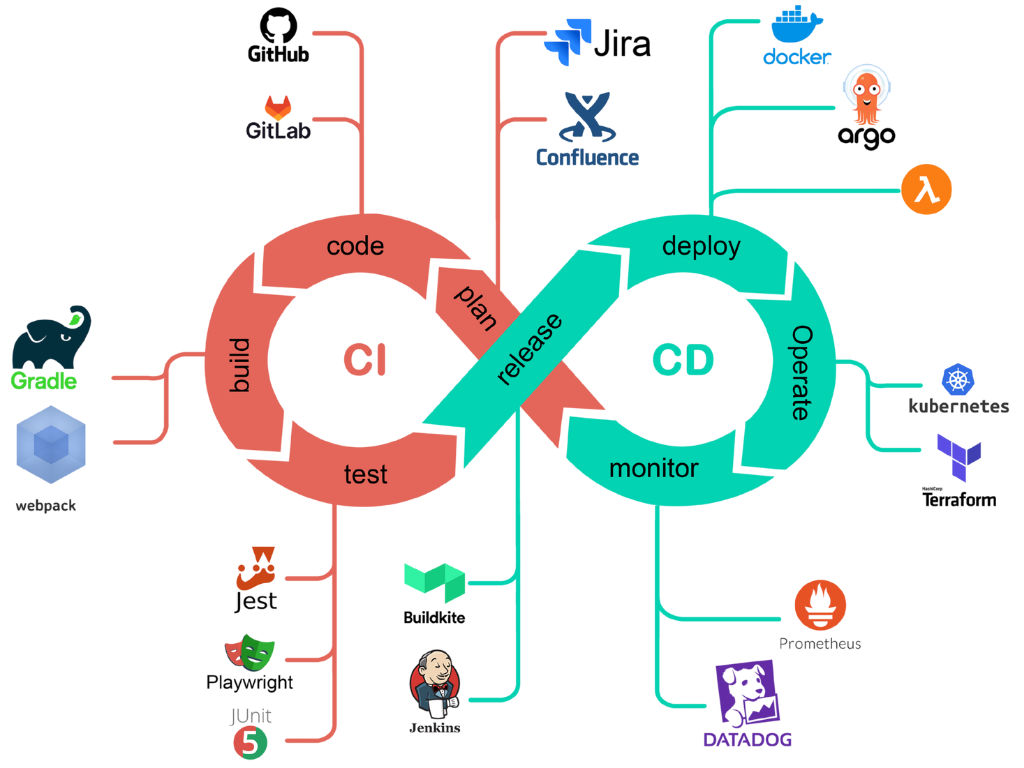
\includegraphics[width=0.8\textwidth]{image9.png}
\caption{DevOps life-cycle and tools}
\label{fig:DevOps life-cycle and tools}
\end{figure}

